\documentclass[xcolor=dvipsnames]{beamer}
\usepackage[T1]{fontenc}
\usepackage[utf8]{inputenc}
\usepackage[english,slovak]{babel}

\usepackage{amsmath}
\usepackage{amsthm}
\usetheme{Pittsburgh}
\useoutertheme{shadow}

\usepackage{graphicx}
\usepackage{caption}
\usepackage{subcaption}

\usepackage[]{algorithm2e}
\usepackage{listings}
 \setbeamercovered{transparent}
 \usepackage{cuted}
\usepackage[export]{adjustbox}
\usepackage{mathtools}

\usepackage{lipsum}
\usepackage{verbatim}
\usepackage{transparent}
\usepackage{framed}
\usepackage{xcolor}

\usepackage{multirow}
\usepackage{colortbl}
\usepackage{lmodern}

\usepackage{movie15}
\usepackage{verbatim}

\usepackage{hyperref}


\newcommand\Wider[2][3em]{%
\makebox[\linewidth][c]{%
  \begin{minipage}{\dimexpr\textwidth+#1\relax}
  \raggedright#2
  \end{minipage}%
  }%
}






\iffalse

\usetheme{Warsaw}

\setbeamercolor{normal text}{fg=white,bg=black!90}
\setbeamercolor{structure}{fg=white}

\setbeamercolor{alerted text}{fg=red!85!black}

\setbeamercolor{item projected}{use=item,fg=black,bg=item.fg!35}

\setbeamercolor*{palette primary}{use=structure,fg=structure.fg}
\setbeamercolor*{palette secondary}{use=structure,fg=structure.fg!95!black}
\setbeamercolor*{palette tertiary}{use=structure,fg=structure.fg!90!black}
\setbeamercolor*{palette quaternary}{use=structure,fg=structure.fg!95!black,bg=black!80}

\setbeamercolor*{framesubtitle}{fg=white}

\setbeamercolor*{block title}{parent=structure,bg=black!60}
\setbeamercolor*{block body}{fg=black,bg=black!10}
\setbeamercolor*{block title alerted}{parent=alerted text,bg=black!15}
\setbeamercolor*{block title example}{parent=example text,bg=black!15}

\fi



%-------------------------------------------------------------------------------------
\title{\color{white} \bf DQN}
\author{\color{white} Michal CHOVANEC, PhD}


%\setbeamertemplate{footline}[frame number]{}
\setbeamertemplate{navigation symbols}{}


\date[EURP]{}
\begin{document}

{
    \usebackgroundtemplate
    {
        \vbox to \paperheight{\vfil\hbox to \paperwidth{\hfil

        {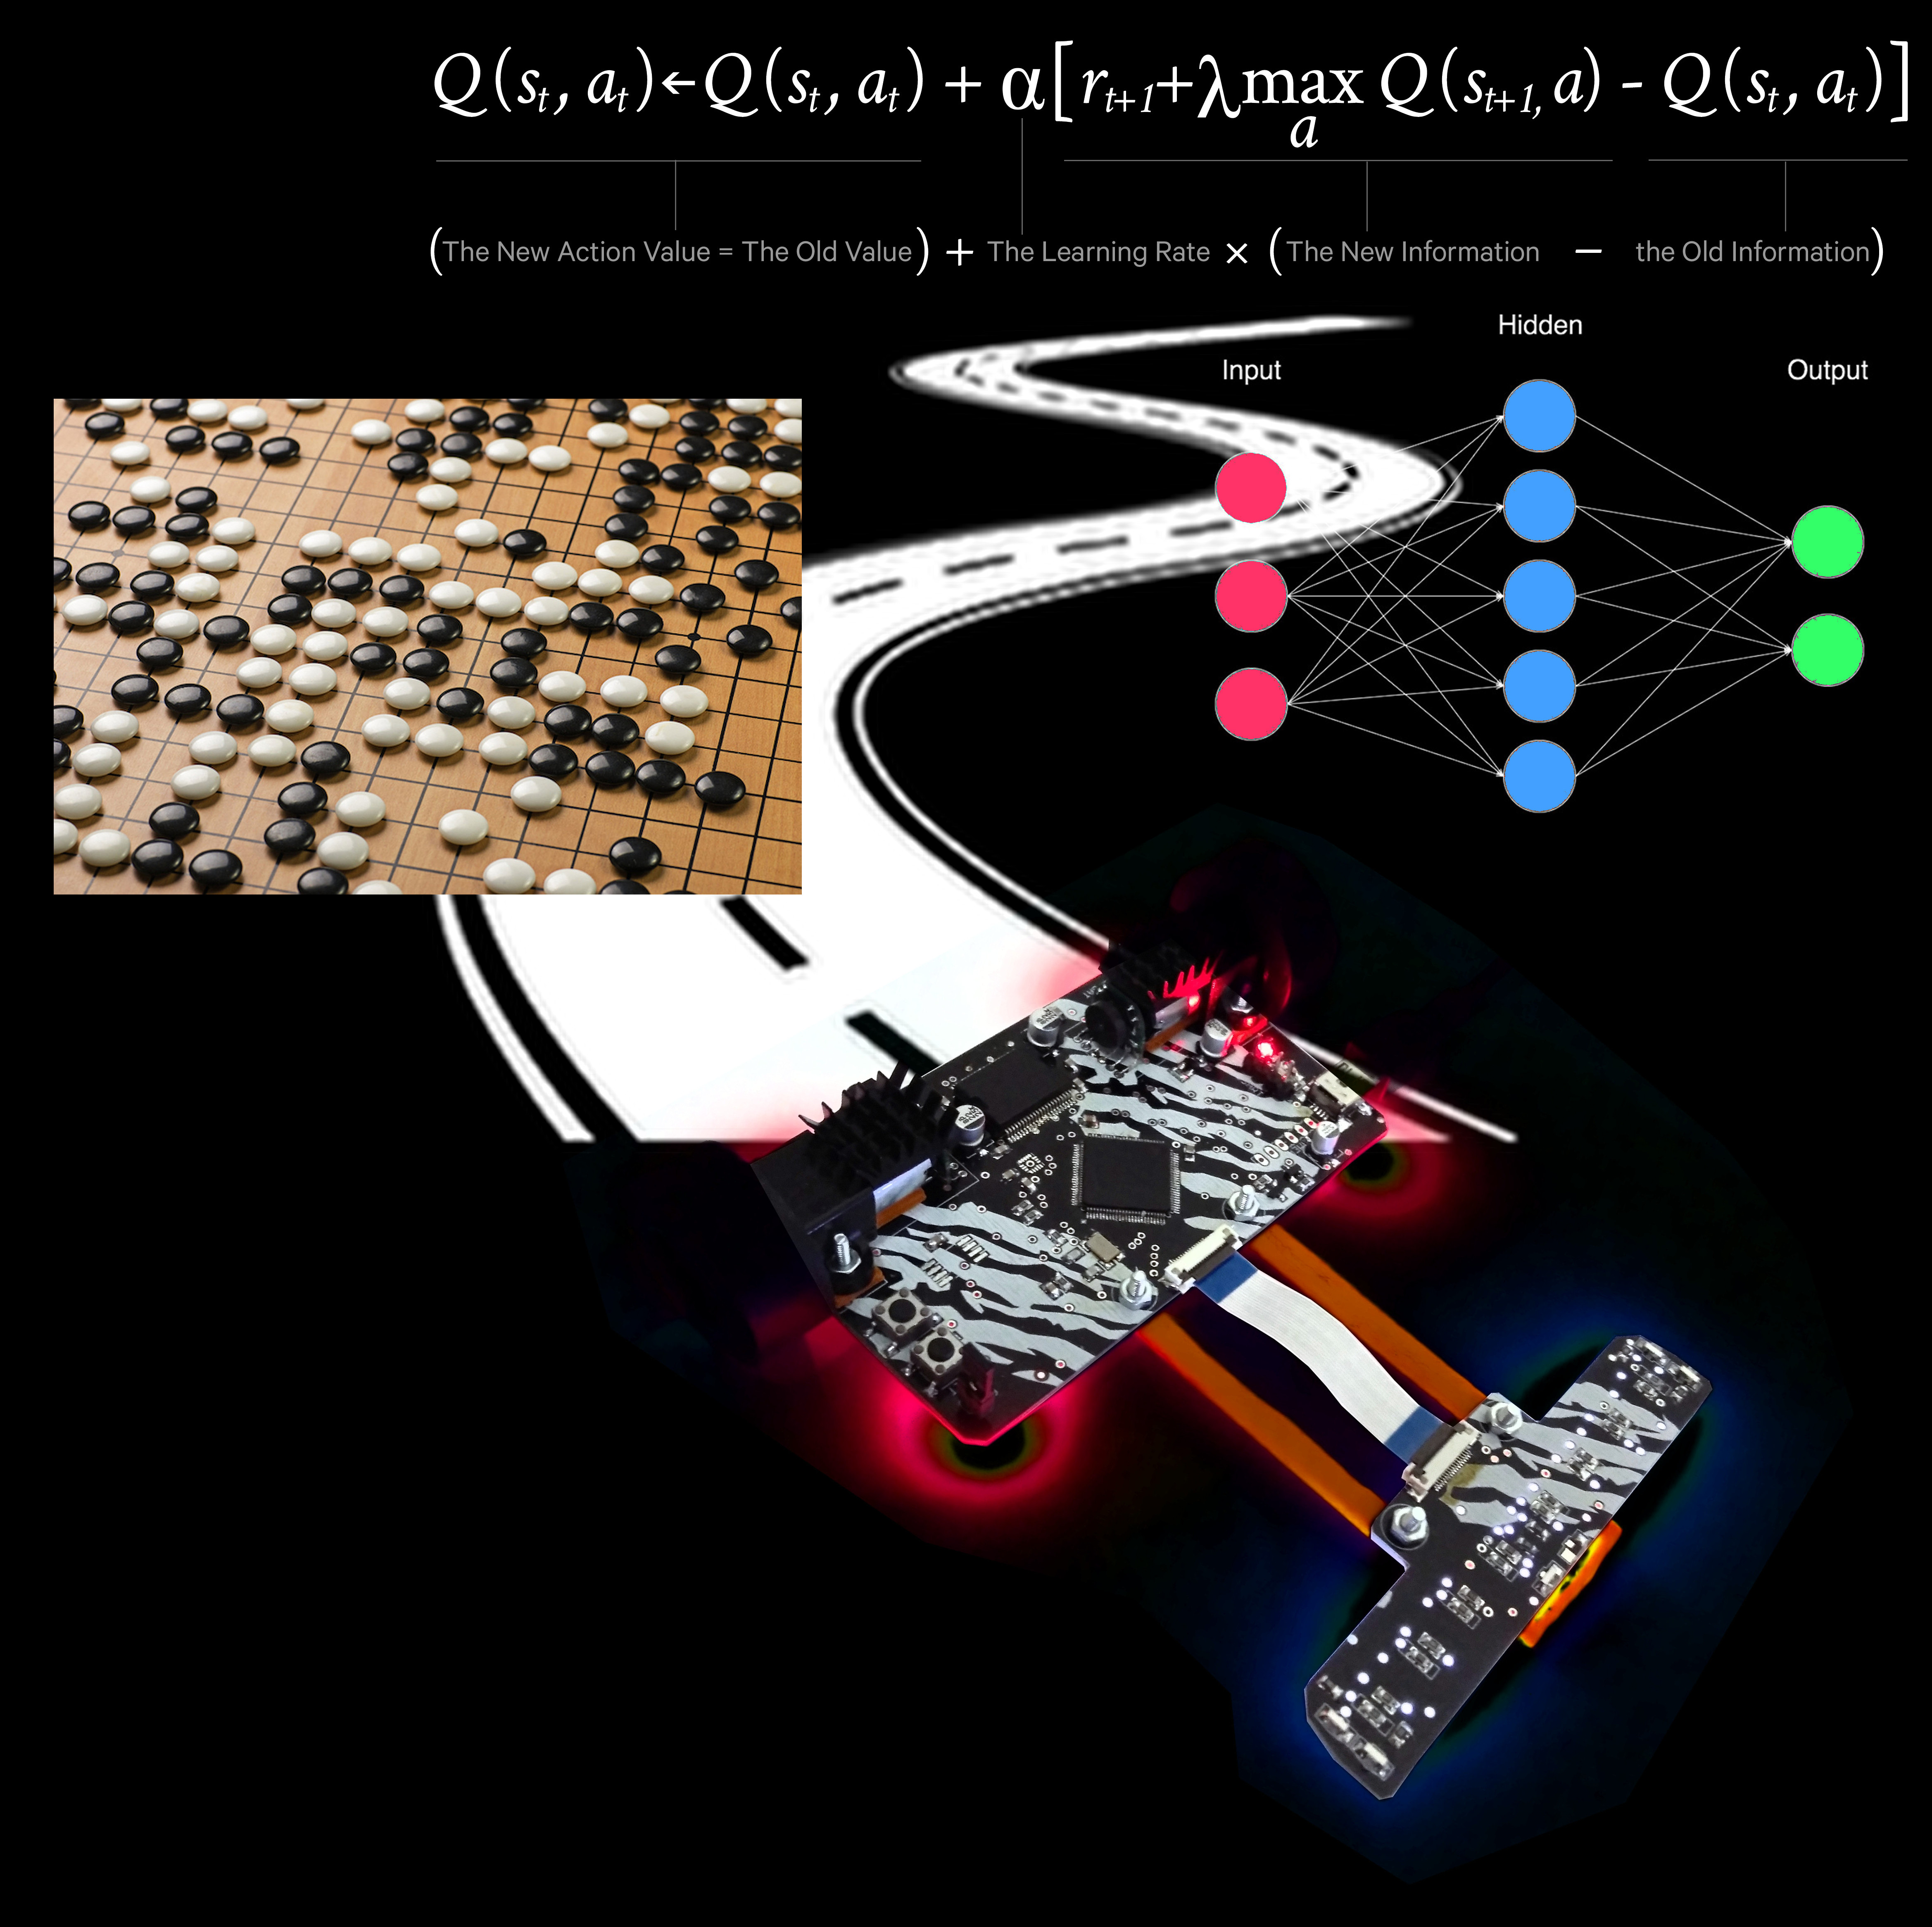
\includegraphics[width=5.05in]{./pictures/rl_square.jpg}}

        \hfil}\vfil}
    }
    \begin{frame}

    %\titlepage


    \centering
     \colorbox{black}
     {
        \begin{minipage}{7cm}
           {\LARGE \color{white} \bf reinforcement learning \\ - pytorch, AI gym} \\
           {\LARGE \color{white} Michal CHOVANEC} \\
       \end{minipage}
     }


    \end{frame}
}

\begin{frame}{\bf reinforcement learning}

\begin{columns}
  \begin{column}{0.5\textwidth}
      \centering
      \includemovie[
        poster,
        autoplay,
        externalviewer,
        inline=false,
        text={ 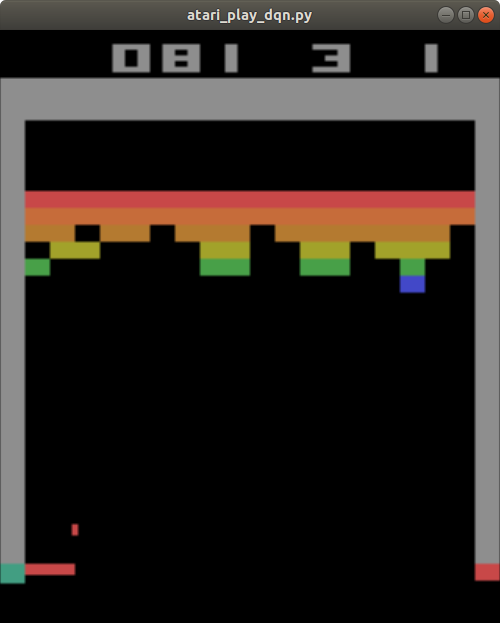
\includegraphics[scale=0.15]{./pictures/breakout.png}}
      ]{3cm}{3.3cm}{./video/rl_atari.mp4}

  \begin{figure}
    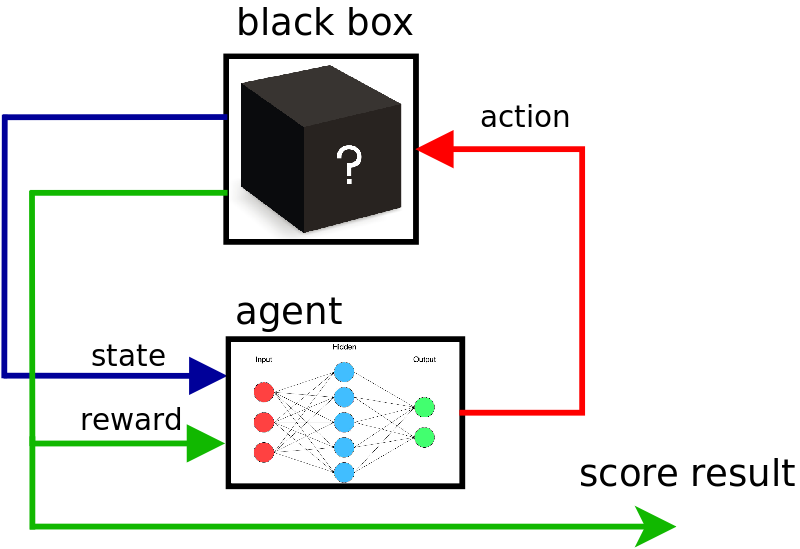
\includegraphics[scale=0.3]{./diagrams/rl_mechanism.png}
  \end{figure}

  \end{column}
  \begin{column}{0.5\textwidth}  %%<--- here

  {\bf
    \begin{itemize}
      \item learning from punishments and rewards
      \item learn to play a game with unknow rules
    \end{itemize}
  }

  \begin{enumerate}
    \item obtain {\bf state}
    \item choose {\bf action}
    \item {\bf execute} action
    \item obtain {\bf reward}
    \item learn from {\bf experiences}, $Q(s, a)$, or $\pi(a|s)$
  \end{enumerate}


  \end{column}
\end{columns}

\end{frame}


\begin{frame}{\bf reinforcement learning}

  \begin{itemize}
    \item supervised - {\bf learning from dataset} : classification, detection, segmentation \\ 
      $\mathcal{L} = (Y_{target} - \hat{Y}_{predicted})^2$, (RMS, crossentropy ...)\\
      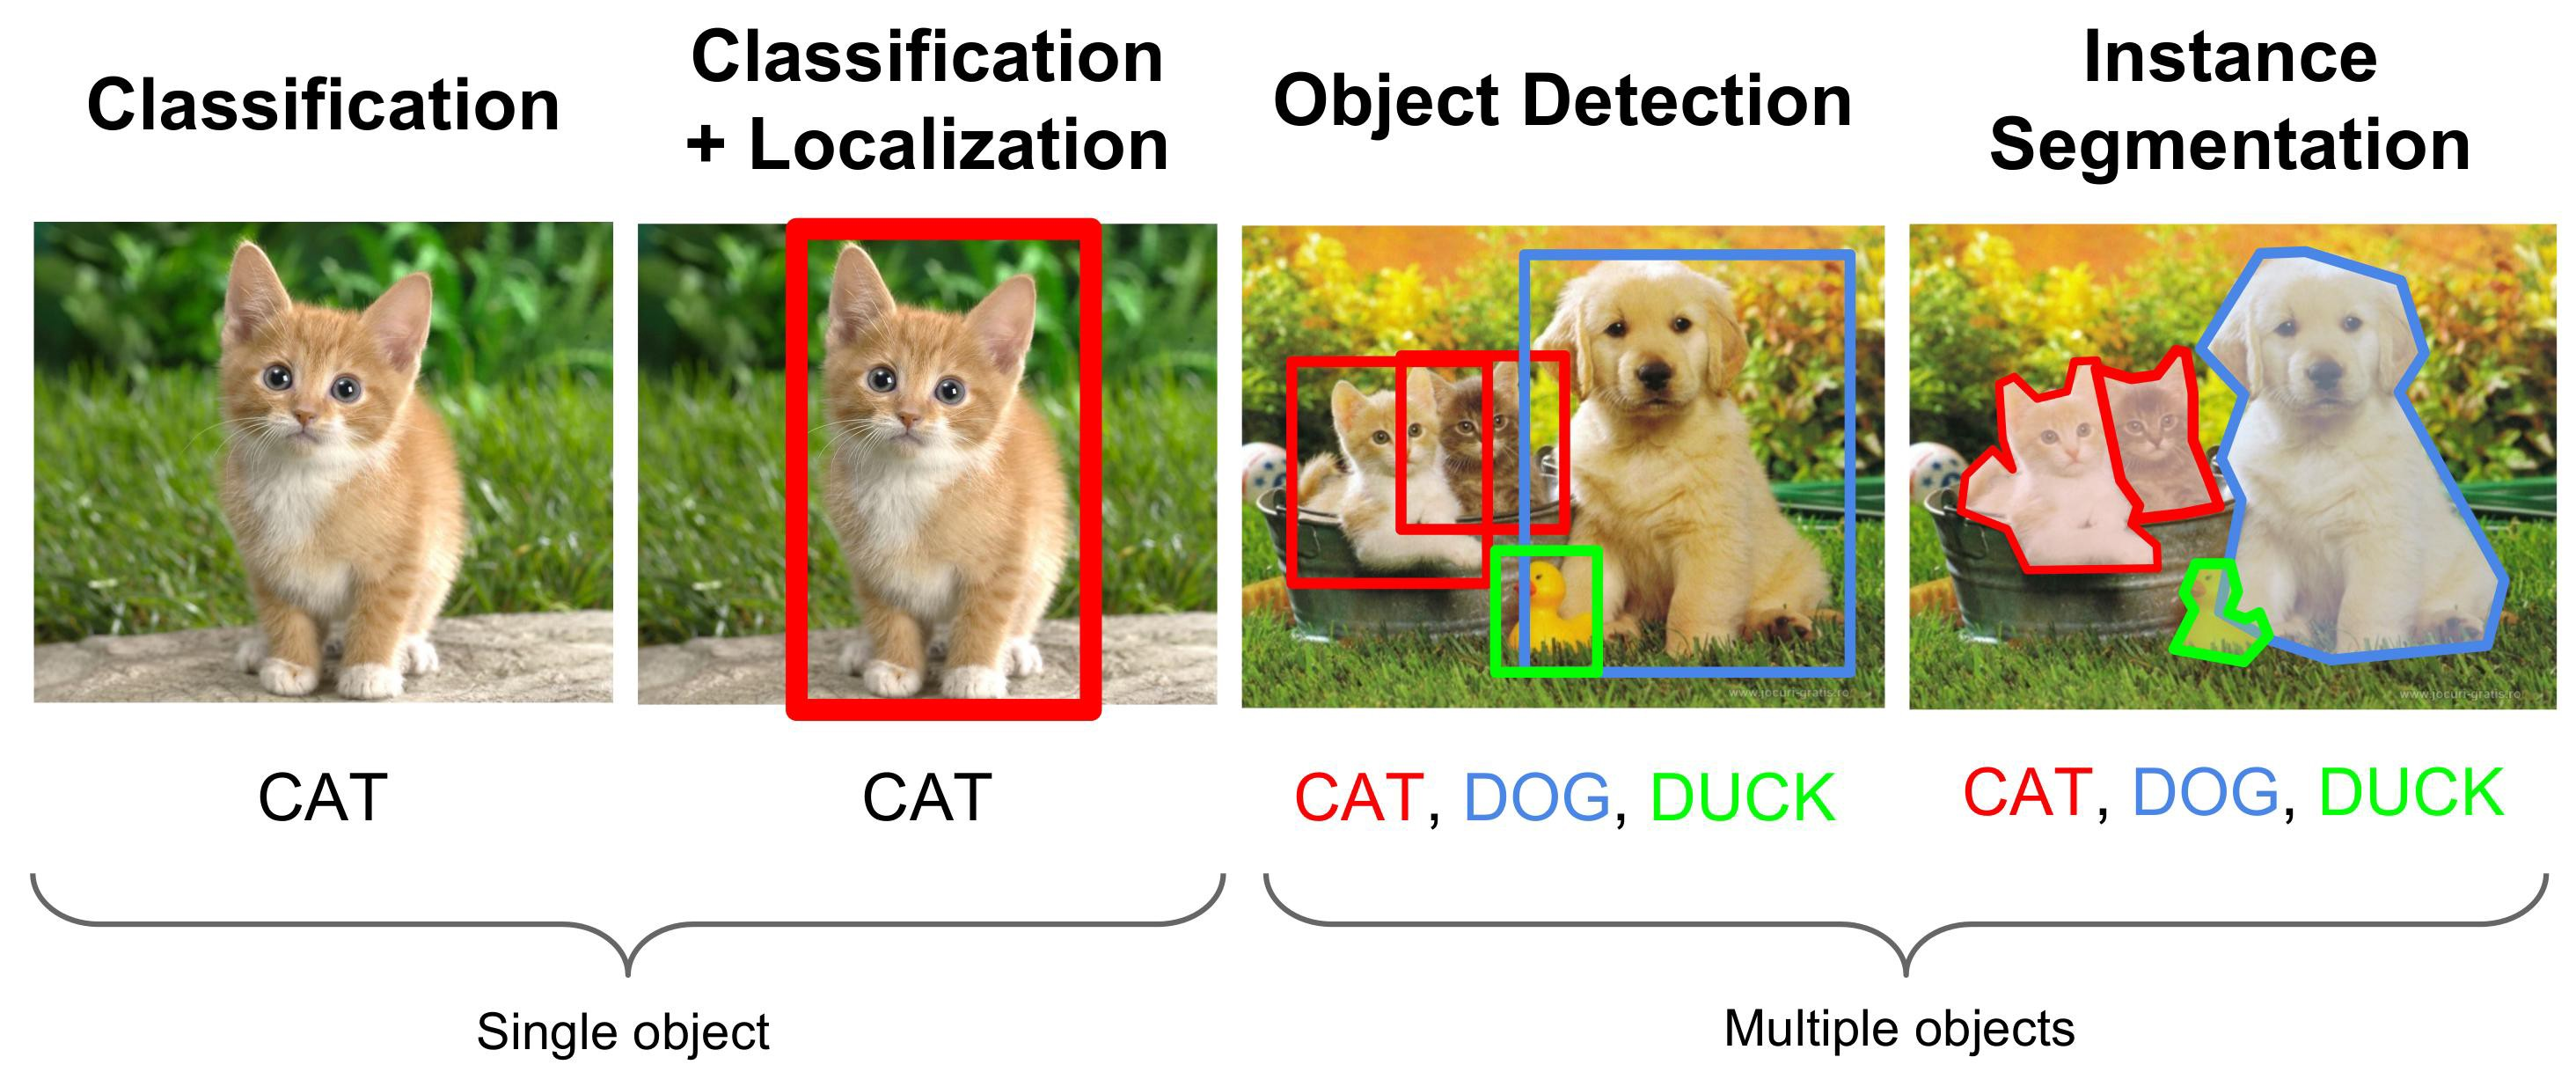
\includegraphics[scale=0.05]{./pictures/image_supervised.jpg}
    \item reinforcement - {\bf learning from experiences} and active interactions
      \begin{itemize} 
        \item expected reward, $Q(s, a)$, value based methods
        \item actions probability, $\pi(a|s)$, policy based methods
      \end{itemize}
  \end{itemize}

\end{frame}




\begin{frame}{\bf Q-learning}


\begin{columns}
  \begin{column}{0.5\textwidth}
    
    $Q(s, a)$ : what is the potential reward in state {\bf s} and action {\bf a}

    \begin{align*}
      Q'(s, a) = R + \gamma \max \limits_{a'} Q(s', a')
    \end{align*}

  \end{column}
  \begin{column}{0.5\textwidth}  %%<--- here

    where \\
    $s$ is state \\
    $a$ is action \\
    $s'$ is next state \\
    $a'$ is best action in next state \\
    $R$ is reward \\
    $\gamma \in \langle 0, 1 \rangle$ is discount factor \\

  \end{column}
\end{columns}

\begin{figure}
  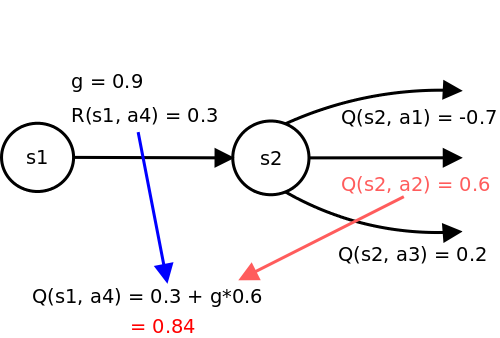
\includegraphics[scale=0.25]{diagrams/q_learning_detail.png}
\end{figure}

\end{frame}




\begin{frame}{\bf weapon of choice}


\begin{columns}

  \begin{column}{0.5\textwidth}  %%<--- here
    \begin{figure}
      
\includegraphics[scale=0.2]{./pictures/pytorch_logo.png}
    \end{figure}

    \begin{figure}
      
\includegraphics[scale=0.3]{./pictures/open_ai_gym.png}
    \end{figure}
  \end{column}
  
  \begin{column}{0.5\textwidth}  %%<--- here


  \begin{enumerate}
    \item pytorch - deep learning library
    \item aigym - tons of environments library

      \begin{enumerate}
        \item atari
        \item classic control
        \item robotics
        \item extensions : super mario, DOOM ...
      \end{enumerate}

  \end{enumerate}


  \end{column}
\end{columns}

\end{frame}



\begin{frame}[fragile]
\frametitle{\bf pytorch - neural network example}

\begin{figure}
  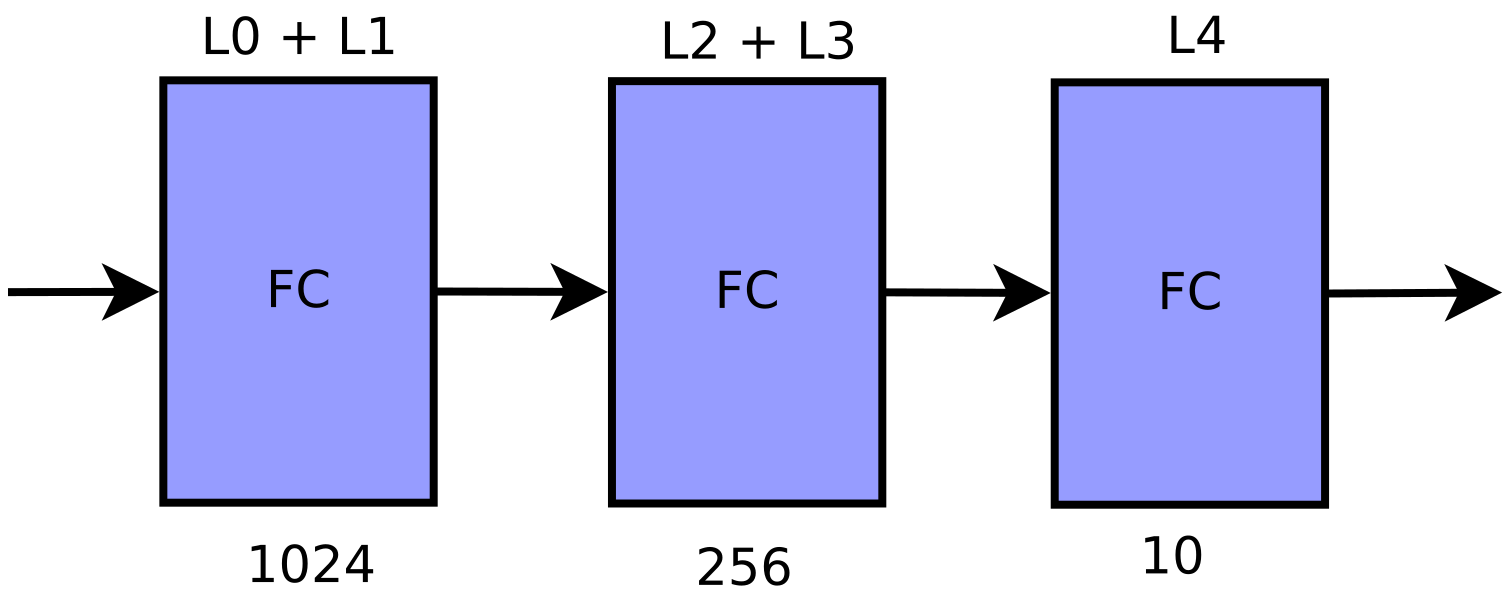
\includegraphics[scale=0.15]{./diagrams/nn_simple.png}
\end{figure}

{\tiny
  \begin{lstlisting}[frame=none, language=Python]
  class MyModel(torch.nn.Module):
      def __init__(self, inputs_count, outputs_count):
          super(MyModel, self).__init__()

          self.l0     = nn.Linear(inputs_count, 1024)
          self.l1     = nn.ReLU()
          self.l2     = nn.Linear(1024, 256)
          self.l3     = nn.ReLU()
          self.l4     = nn.Linear(256, outputs_count)

      def forward(self, input):
          x = input

          x = self.l0.forward(x)
          x = self.l1.forward(x)
          x = self.l2.forward(x)
          x = self.l3.forward(x)
          x = self.l4.forward(x)

          return x
  \end{lstlisting}
}

\end{frame}




\begin{frame}[fragile]
\frametitle{\bf pytorch - neural network example - training}

{\tiny
  \begin{lstlisting}[frame=none, language=Python]
    inputs_count  = 768
    outputs_count = 10
    batch_size    = 32

    #create model
    model = MyModel(inputs_count, outputs_count)

    #create solver, use ADAM, learning rate = 0.001
    optimizer      = torch.optim.Adam(model.parameters(), lr= 0.001)

    #some random data, just example
    x_input     = torch.rand((batch_size, inputs_count))
    y_target    = torch.rand((batch_size, outputs_count))

    #network output
    y_predicted = model.forward(x_input)



    #clear gradients
    optimizer.zero_grad()

    #compute loss, RMS
    loss   = ((y_target - y_predicted)**2).mean()

    #gradient backpropagation
    loss.backward()

    #update weights
    optimizer.step()
  \end{lstlisting}
}


\end{frame}





\begin{frame}[fragile]
\frametitle{\bf pytorch - neural network crazy example}

\begin{columns}

  \begin{column}{0.5\textwidth}  %%<--- here

    {\tiny
      \begin{lstlisting}[frame=none, language=Python]
      class CrazyModel(torch.nn.Module):
          def __init__(self, inputs_count, outputs_count):
              super(CrazyModel, self).__init__()

              self.l0 = nn.Linear(inputs_count, 1024)
              self.l1 = nn.ReLU()

              self.l0B = nn.Linear(inputs_count, 256)
              self.l1B = nn.Sigmoid()

              self.l2 = nn.Linear(1024, 256)
              self.l3 = nn.ReLU()

              self.l4 = nn.Linear(256, outputs_count)

          def forward(self, input):
              x = self.l0.forward(input)
              x = self.l1.forward(x)

              xb = self.l0B.forward(input)
              xb = self.l1B.forward(xb)

              x = self.l2.forward(x)
              x = self.l3.forward(x)
              x = self.l4.forward(x*(xb - 0.5))

              return x
      \end{lstlisting}
    }

  \end{column}

  
  \begin{column}{0.5\textwidth}  %%<--- here

    \begin{figure}
      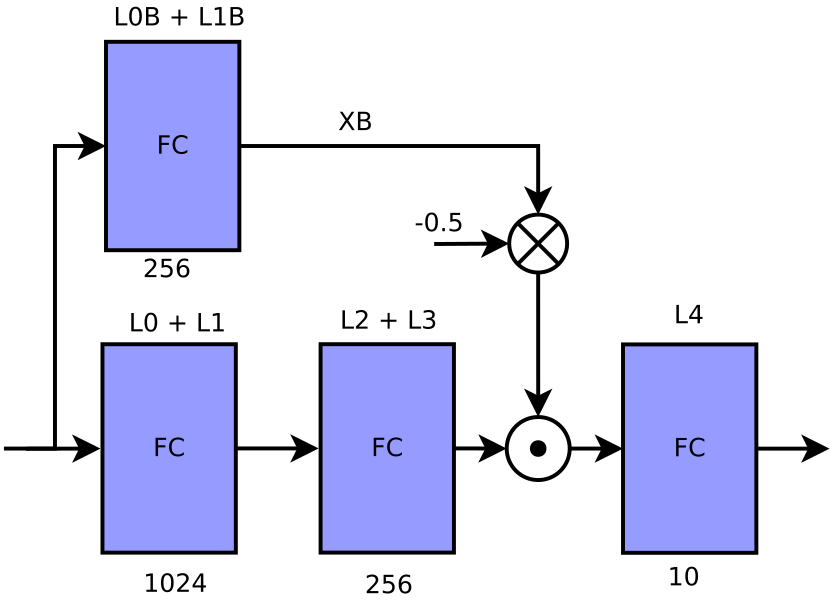
\includegraphics[scale=0.15]{./diagrams/nn_crazy.png}
    \end{figure}

  \end{column}
\end{columns}


\end{frame}





\begin{frame}[fragile]
\frametitle{\bf open AI gym - usage example}




\begin{columns}
  \begin{column}{0.3\textwidth}
    
    \begin{figure}
      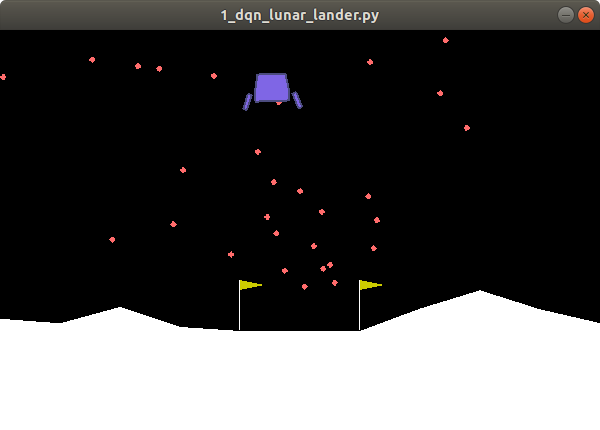
\includegraphics[scale=0.2]{./pictures/lunar_lander.png}
    \end{figure}

  \end{column}
  \begin{column}{0.3\textwidth}  %%<--- here

    \begin{figure}
      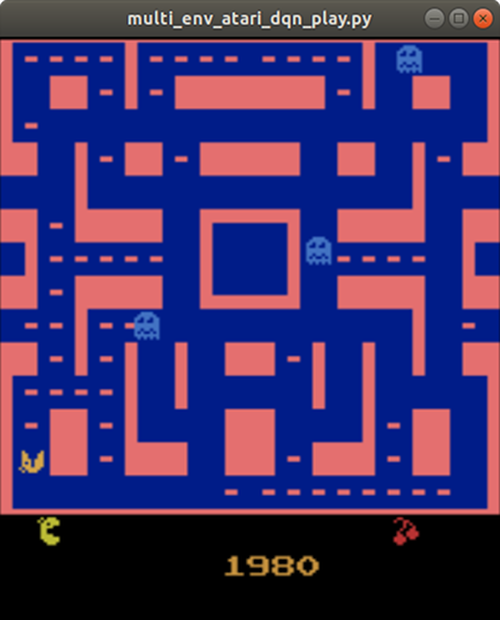
\includegraphics[scale=0.15]{./pictures/pacman.png}
    \end{figure}

  \end{column}


  \begin{column}{0.3\textwidth}  %%<--- here

    \begin{figure}
      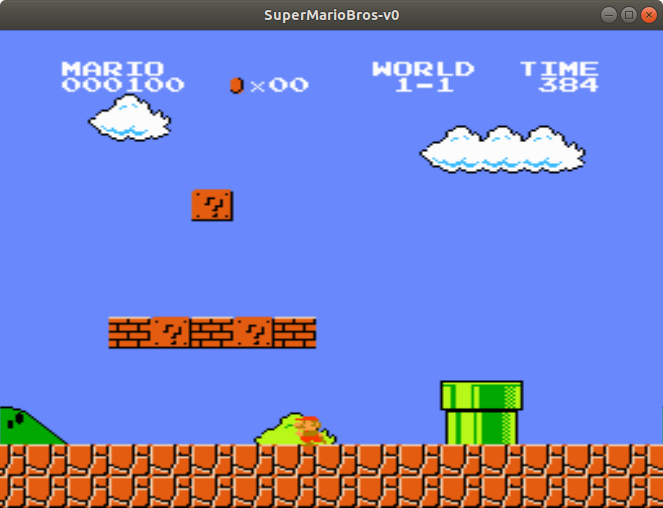
\includegraphics[scale=0.16]{./pictures/supermario.png}
    \end{figure}

  \end{column}
\end{columns}



    {\tiny
      \begin{lstlisting}[frame=none, language=Python]
      import numpy
      import time
      import gym

      env = gym.make("LunarLander-v2")
      state = env.reset()

      actions_count   = env.action_space.n


      while True:
          action = numpy.random.randint(actions_count)
          state, reward, done, info = env.step(action)
          env.render()
          time.sleep(0.01)

      \end{lstlisting}
    }


\end{frame}


\begin{frame}[fragile]
\frametitle{\bf deep Q network}

  \begin{figure}
      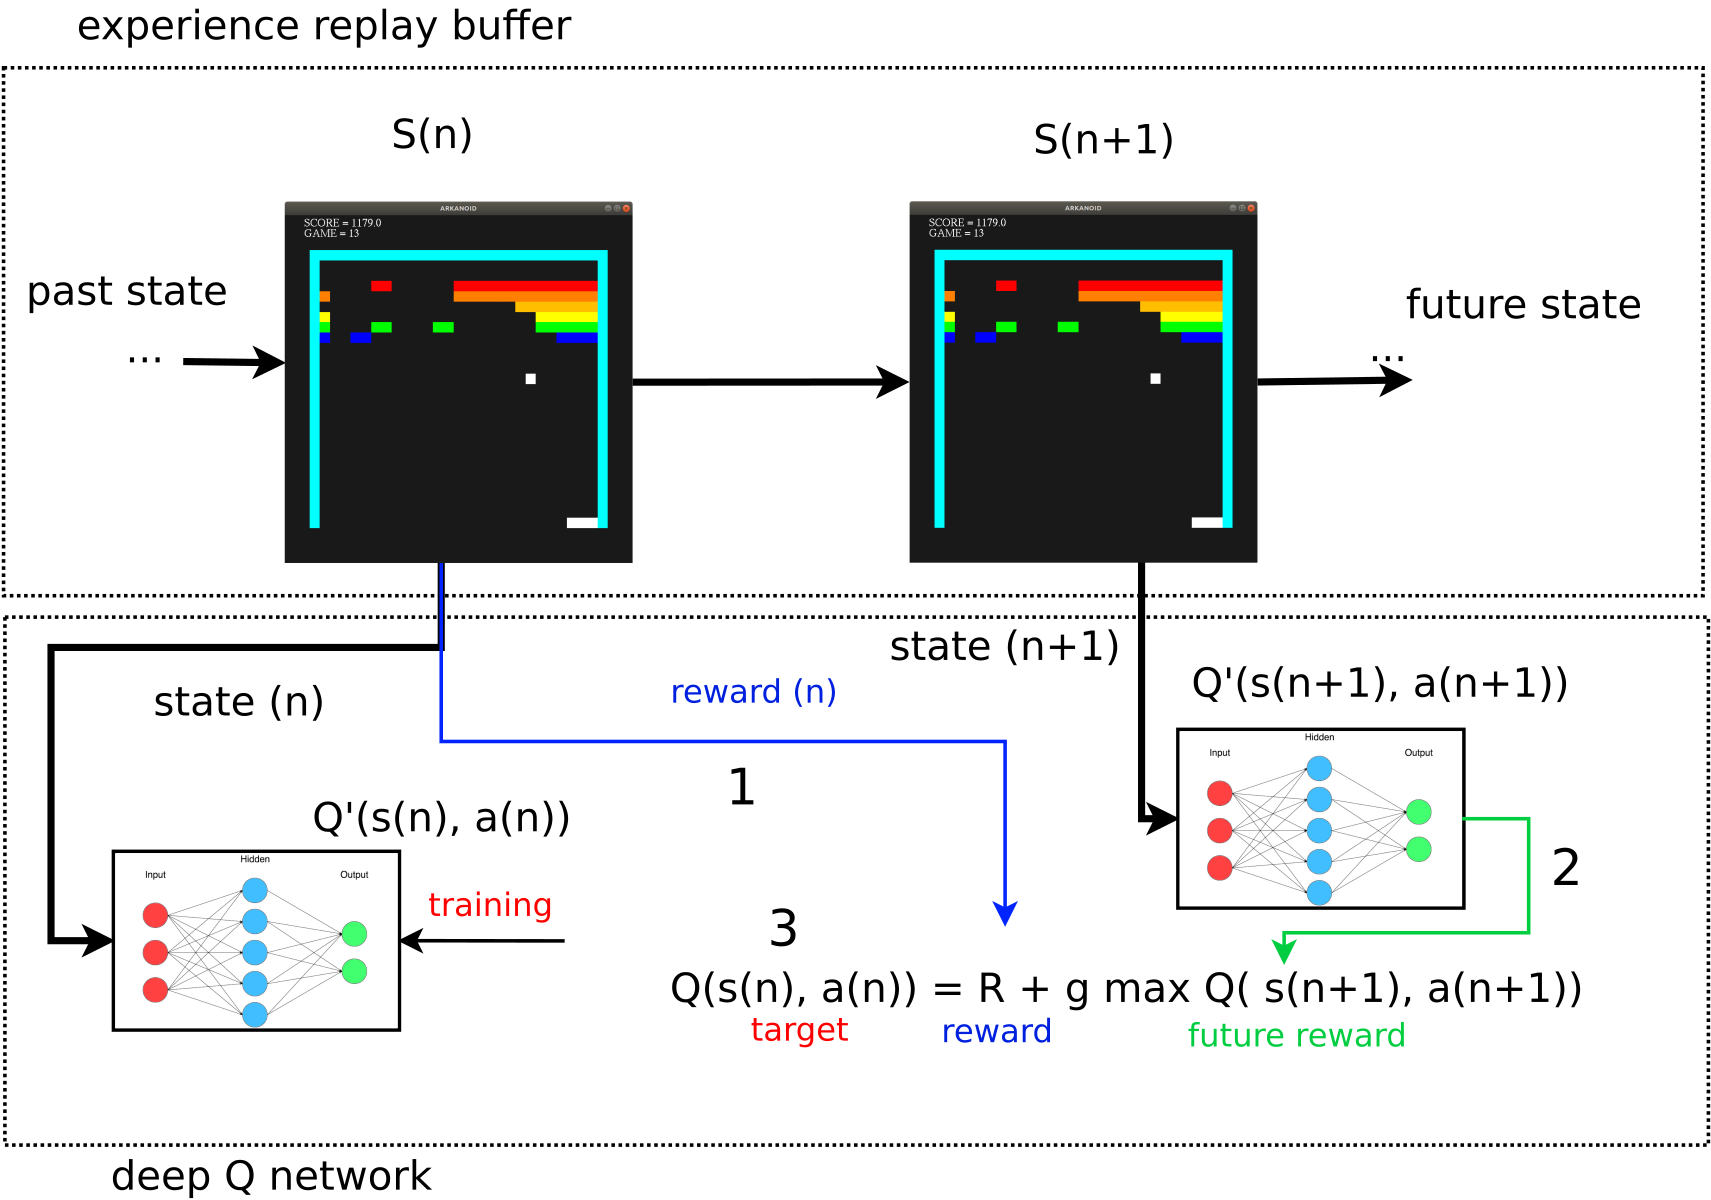
\includegraphics[scale=0.12]{./diagrams/dqn_machism.png}
  \end{figure}


  \begin{columns}


  \begin{column}{0.5\textwidth}  %%<--- here

  {\tiny
      \begin{lstlisting}[frame=none, language=Python]
       def train_model():
          state, q_target = get_random_batch(batch_size)
            
          q_predicted = model.forward(state)

          optimizer.zero_grad()

          loss = (q_target - q_predicted)**2
          loss = loss.mean() 
          loss.backward()
          optimizer.step()

      \end{lstlisting}
    }

    \end{column}
  

  \begin{column}{0.5\textwidth}  %%<--- here

    \begin{align*}
      Q'(s, a) &= R + \gamma \max \limits_{a'} Q(s', a') \\
      \mathcal{L} &= (R + \gamma \max \limits_{a'} \hat{Q}(s', a') - \hat{Q}(s, a))^2
    \end{align*}

  \end{column}


  
\end{columns}



\end{frame}




\begin{frame}{\bf Q\&A - consultations on Rysy Hut 2250 m.a.s.l.}
 \vspace{-6mm}
\begin{figure}
  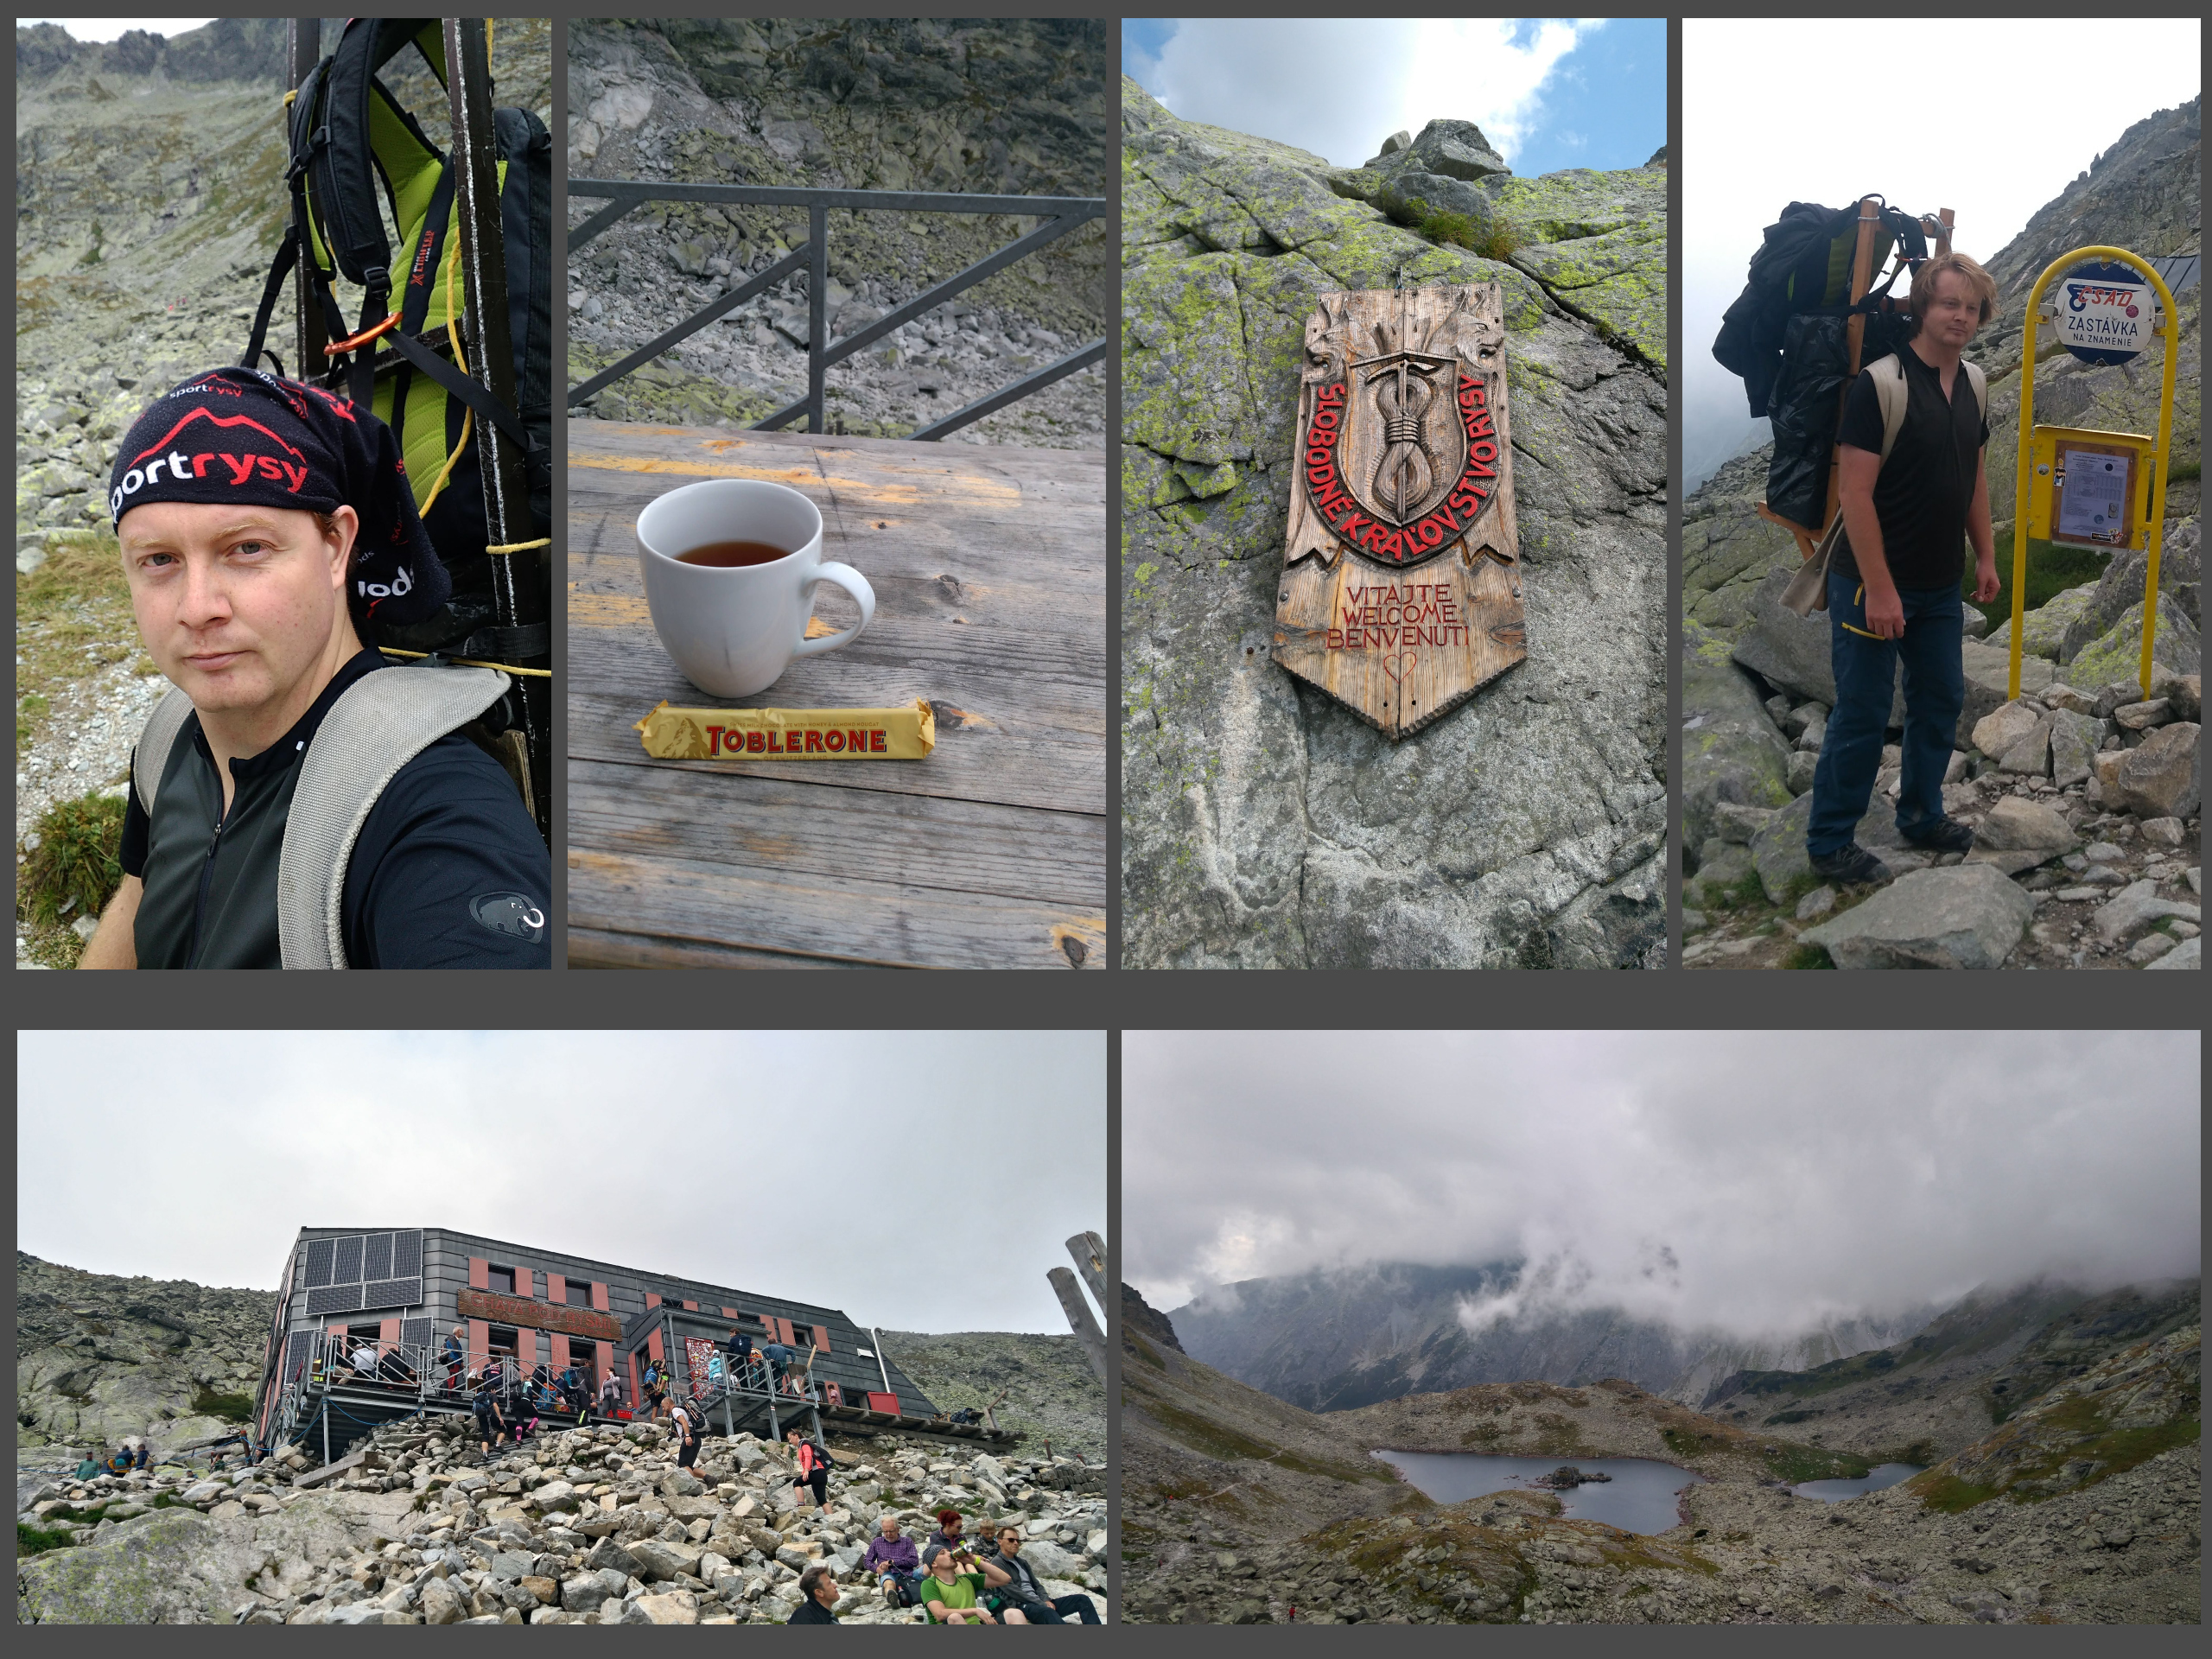
\includegraphics[scale=0.5]{./pictures/me_rysy.jpg}
\end{figure}

\end{frame}




\end{document}
